\documentclass[a4paper, 14pt]{extarticle}

\usepackage{amsmath}
\usepackage{amssymb}
\usepackage{amsthm}
\usepackage{commath}
\usepackage[margin=0.5in]{geometry}
% \usepackage{lexend}
\usepackage{microtype}
\usepackage{parskip}
\usepackage{tikz}
\usepackage{tikz-cd}
\usepackage{tkz-euclide}
\usepackage{xparse}

\usetikzlibrary{calc,angles,quotes, positioning, shapes.geometric}

\theoremstyle{definition}
\newtheorem{dfn}{Definition}
\newtheorem{clm}{Claim}
\newtheorem{asn}{Assertion}
\newtheorem{thm}{Theorem}
\newtheorem{prb}{Problem}
\newtheorem{ans}{Answer}
\newtheorem{lm}{Lemma}
\newtheorem{rmk}{Remark}
\newtheorem{crl}{Corollary}
\newtheorem{ex}{Exercise}
\newtheorem{xmp}{Example}

\newcommand{\titleheader}[1]{\begin{centering}
\begin{LARGE}
\textbf{#1}
\end{LARGE}\\
\hrulefill

\vspace{-1.25\baselineskip}
\hrulefill
\end{centering}\\\\}

\def\changemargin#1#2{\list{}{\rightmargin#2\leftmargin#1}\item[]}
\let\endchangemargin=\endlist

\NewDocumentEnvironment{smrg}{}{\begin{changemargin}{0.5cm}{0.5cm}}{\end{changemargin}}

\NewDocumentEnvironment{SWP}{m m}
{%
  \vspace{-.9cm}%
  \begin{changemargin}{0.5cm}{0.5cm}%
  \noindent#1~#2
  \par
  \textbf{Proof.} 
}
{%
  \qed
  \end{changemargin}
}

\NewDocumentEnvironment{SNP}{m}
{%
  \vspace{-.9cm}%
  \begin{changemargin}{0.5cm}{0.5cm}%
  \noindent#1
}
{%
  \end{changemargin}
}

\newcommand{\bb}[1]{\mathbb{#1}}
\newcommand{\st}{\space \mid \space}
\newcommand{\union}[1]{\displaystyle\mathop{\cup}\limits_{#1}}
\newcommand{\intersect}[1]{\displaystyle\mathop{\cap}\limits_{#1}}
\newcommand{\paran}[1]{\left ( {#1} \right )}
\newcommand{\contra}{$\rightarrow\!\leftarrow$}
\newcommand{\kvec}[2]{({#1}_1 \dots {#1}_{#2})}
\newcommand{\pf}{\textbf{Proof.} }

\newcommand{\AnswerSection}{
    \newpage
    \section*{Answers to Exercises}
    \textit{The following are brief solutions or hints. You are encouraged to review the exercises before checking the answers.}
}
\begin{document}
\titleheader{Intermediate Value Theorem}
\textbf{Prereqs} RA-11

Let's put our definition of continuity through a litmus test. Suppose $f$ is a continuous function in the pen and paper sense and is defined on a closed interval $[a, b]$.

Suppose that $f(a) > 0$ and $f(b) < 0$. Is it true that $f(c) = 0$ for some $c \in (a, b)$?
\begin{center}
\begin{tikzpicture}{x=3cm}{y=3cm}
  \draw[->] (-1,0) -- (6,0) node[right] {$x$};
  \draw[->] (0,-1.5) -- (0,2.5) node[above] {$y$};

  \draw[domain=1.5:4.5, smooth, variable=\x, red, thick] 
    plot ({\x}, {sin(deg(\x))});

  \pgfmathsetmacro{\ya}{sin(deg(1.5))}
  \node at (1.5, \ya) [above] {$(a, f(a))$};
  \pgfmathsetmacro{\yb}{sin(deg(4.5))}
  \node at (4.5, \yb) [below] {$(b, f(b))$};
\end{tikzpicture}\\
Does a continuous curve hit the $x-$axis if it starts above and ends below?
\end{center}
Intuitively -- yes! If I have to reach below the $x-$axis from above, can I do that without lifting my pen? Absolutely not. Does our definition capture this?

\begin{SWP}{\thm}{(Bolzano's Theorem) If $f: [a, b] \rightarrow \bb R$ is continuous with $f(a) < 0$ and $f(b) > 0$ (or vice versa), then $f(c) = 0$ for some $c$ in $(a, b)$}Consider the set$$S = \{x \in [a, b] \st f(x) \leq 0\}$$
Observe that $a \in S$ therefore $S$ is nonempty. Also since $S \subset [a, b]$ therefore every $x \in S$ is smaller than $b$. One can even say $S$ is bounded above by $b$.

Whenever a nonempty set is bounded above, it has a least upper bound. Let it be $\alpha$ in this case. Intuitively, $\alpha$ is the last possible value of $x$ for which $f(x) \leq 0$. Can we claim that $f(\alpha) = 0$?

Since $\alpha$ is the least upper bound of $S$, there is a sequence $\{a_n\} \subset S$ such that $a_n \rightarrow \alpha$ $(\ast)$. Since $f$ is continuous, $f(a_n) \rightarrow f(\alpha)$. But all of $f(a_n)$ are $\leq 0$, therefore $f(\alpha) \leq 0$ $(\ast \ast)$. Here we use the ``least'' part of the least upper bound.

Since $f(\alpha) \leq 0$, we conclude that $\alpha \neq b$. Combining with $\alpha \leq b$ gives $\alpha < b$. Now we construct another sequence which approaches $\alpha$ from the right. Take $c_n = \alpha + \dfrac{b - \alpha}{n}$. Here, $c_1 = b$ and the sequence monotonically decreases to $\alpha$.

Again, $c_n \rightarrow \alpha$ and thus $f(c_n) \rightarrow f(\alpha)$. Here we will exploit the ``upper bound'' property. Since $c_n > \alpha$ and $\alpha$ is an upper bound of $S$, none of the $c_n$ lie in $S$ and hence $f(c_n) > 0$. Further, $f(c_n) \rightarrow f(\alpha)$ gives $f(\alpha) \geq 0$. Thus $f(\alpha) = 0$.
\end{SWP}
Our definition passes the litmus test!
% \newpage
\begin{SNP}{\crl}{(Intermediate Value Theorem) Let $f:[a,b] \rightarrow \bb R$ be continuous and let $k \in \bb R$ be such that $f(a) < k$ and $f(b) > k$ (or vice versa). Then $f(c) = k$ for some $c \in (a, b)$}
\end{SNP}

Observe that I have used results $(\ast)$ and $(\ast \ast)$ in the proof, which I'll properly state and leave out as exercises.

\begin{SNP}{\ex}{Let $S$ be a nonempty bounded subset of $\bb R$ and $\alpha$ be its least upper bound. Show that there is a sequence $a_n$ with all its terms in $S$ and $a_n \rightarrow \alpha$}.
\end{SNP}
\begin{SNP}{\ex}{Let $\{a_n\}$ be a sequence such that $a_n \rightarrow L$ and $a_n > 0$ for every $n$. Show that $L \geq 0$ and give an example of a sequence where $L = 0$}.
\end{SNP}
\AnswerSection
\ans Since $\alpha$ is the least upper bound, $\alpha - \frac{1}{n}$ cannot be an upper bound of $S$, therefore there is some $a_n \in S$ such that
$$
\alpha - \dfrac 1 n \leq a_n \leq \alpha
$$
where the first inequality is because $\alpha - \frac 1 n$ is not an upper bound of $S$, and the second one is because $\alpha$ is an upper bound of $S$.

Now we need to check if the sequence converges to $\alpha$. Let $\epsilon > 0$ be given, and take $N$ to be such that $N > \dfrac{1}{\epsilon}$ (such $N$ exists by Archimedean property). Take $n \geq N$, then
\begin{align*}
n &\geq \dfrac{1}{\epsilon}\\
\implies \epsilon &\geq \dfrac 1 n\\
\implies \alpha - \epsilon &\leq \alpha - \dfrac 1 n 
\end{align*}
Thus whenever $n \geq N$, we get
$$
\alpha - \epsilon \leq \alpha - \dfrac{1}{N} \leq \alpha - \dfrac{1}{n} \leq a_n \leq \alpha
$$
Therefore $a_n \rightarrow \alpha$\qed
\ans Let $a_n > 0$ for every $n$ and suppose $a_n \rightarrow \alpha$. Suppose for contradiction that $\alpha < 0$. Let the distance between $\alpha$ and $0$ be $d$ (i.e, $\alpha = -d$ with $d > 0$).

The idea is, if all $a_n > 0$ and $\alpha < 0$, then $\alpha$ is sufficiently seperated from the sequence. Just take $\epsilon = d$. Can the sequence fall within $d$ distance of $\alpha$? No!

\begin{center}
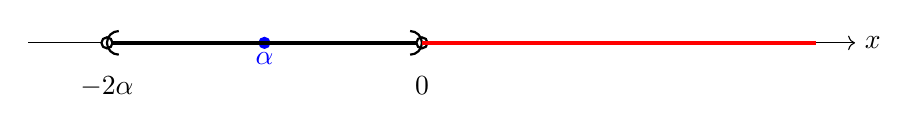
\begin{tikzpicture}[x=1cm, y=1cm]
  \draw[->] (-5,0) -- (5.5,0) node[right] {$x$};

  \def\alph{-2}
  \def\leftpt{2*\alph}
  \def\rightpt{0}

  \filldraw[blue] (\alph,0) circle (2pt) node[below] {$\alpha$};

  \draw[very thick] (\leftpt, 0) -- (\rightpt, 0);
  \filldraw[fill=white, draw=black, thick] (\leftpt, 0) circle (2pt);
  \filldraw[fill=white, draw=black, thick] (\rightpt, 0) circle (2pt);

  \draw[thick] (-3.85, -0.15) arc (270:90:0.15);
  \draw[thick] (-0.15, -0.15) arc (-90:90:0.15);

  \node[below] at (\leftpt, -0.3) {$-2\alpha$};
  \node[below] at (\rightpt, -0.3) {$0$};

  \draw[red, ultra thick] (0,0) -- (5,0);
\end{tikzpicture}\\
The sequence lies in the red section and cannot touch the $\abs{\alpha}-$neighborhood of $\alpha$
\end{center}
Therefore $\alpha \geq 0$. An example where $\alpha = 0$ is the classic $a_n = \frac 1 n$

\end{document}